\documentclass[aip,reprint,groupedaddress,onecolumn,superscriptaddress]{revtex4-2}
\usepackage{graphicx}% Include figure files
\usepackage{dcolumn}% Align table columns on decimal point
\usepackage{bm}% bold math
\usepackage{amsmath}
\usepackage{siunitx}
\usepackage{enumitem}
\usepackage{booktabs} % For better tables

\begin{document}

\title{Precision Refractive Index Measurement at 1762 nm}
%\title{Bullet-Point: Quantum-Traceable Refractometry for Barium-Ion Networks}
\date{\today}

\maketitle

% ============================================
% EXECUTIVE SUMMARY
% ============================================
\section{Executive Summary}

\subsection{Core Innovations}
\begin{itemize}
    \item \textbf{Dual-Wavelength Interferometry}: Modified NIST LM10 \cite{fox1999reliable} design for precision refractive index measurement in the visible to mid-infrared wavelength range
    \item \textbf{SI-Traceable Metrology}: Direct linkage to atomic frequency standards enables high-accuracy environmental monitoring
    \item \textbf{Wavelength-Specific Calibration}: Focused measurement at \SI{1762}{\nano\meter} to address data gaps in existing atmospheric models
\end{itemize}

\subsection{Key Results}
\begin{itemize}
    \item \textbf{Precision Refractive Index Model}: Developed and validated a wavelength-specific refractive index model at \SI{1762}{\nano\meter}, achieving $\delta n \sim 1.82\times10^{-7}$ residual precision through dual-wavelength interferometric measurements.
    \item \textbf{Database Calibration}: Calibrated existing atmospheric models (Ciddor\cite{ciddor1996refractive}, Edlén\cite{edlen1966refractive}, Mathar\cite{mathar2007refractive}) at the \SI{1762}{\nano\meter} wavelength, addressing a critical data gap for applications requiring precise refractive index values at specific wavelengths.
    \item \textbf{Enhanced Humidity Sensitivity}: Identified a \SI{12.4}{\percent} enhanced humidity sensitivity at \SI{1762}{\nano\meter} relative to standard models, consistent with Kramers-Kronig predictions\cite{perakis2016vibrational} near water absorption lines\cite{kochanov2016hitran}.
\end{itemize}

% ============================================
% SYSTEM OVERVIEW
% ============================================
\section{System Overview}

\subsection{Dual-Wavelength Interferometric Refractometer}
\begin{itemize}
    \item \textbf{Core Design}: Michelson interferometer operating at \SI{780}{\nano\meter} (reference) and \SI{1762}{\nano\meter} (probe)
    \item \textbf{Operating Principle}: Simultaneous fringe counting with common-mode environmental noise rejection
    \item \textbf{Key Features}:
    \begin{itemize}
        \item Ratio-metric approach cancels mechanical vibrations
        \item \SI{4.2}{\meter} optical path difference for long-path-length measurements %metropolitan-scale representation
        \item Air-floated mirror stage for vibration isolation
    \end{itemize}
\end{itemize}

\subsection{Quantum Frequency References}
\begin{itemize}
    \item \textbf{780 nm Reference}: semiconductor laser stabilized via saturation absorption spectroscopy of $^{87}$Rb
    \begin{itemize}
        \item Frequency stability: \SI{\sim100}{\kilo\hertz} linewidth (homodyne measurement \cite{ludvigsen1998laser})
        \item Uncertainty contribution: $\delta n \sim 10^{-10}$ (short-term), $\delta n \sim 10^{-9}$ (medium-term)
    \end{itemize}
    
    \item \textbf{1762 nm Probe}: semiconductor laser stabilized to ULE (ultralow-expansion) cavity referenced to single trapped $^{138}$Ba$^+$ ion
    \begin{itemize}
        \item Frequency stability: $<$\SI{1}{\kilo\hertz}
        \item Uncertainty contribution: $\delta n < 10^{-12}$ (all time scales)
    \end{itemize}
\end{itemize}

\subsection{Supporting Infrastructure}
\begin{itemize}
    \item \textbf{Environmental Monitoring}: BME280 sensors were co-located with the optical beam path to minimize spatial mismatch between environmental sensing and optical measurements. The sensors exhibit the following uncertainty specifications:
    \begin{itemize}
        \item Temperature: \SI{\pm 1}{\degreeCelsius} uncertainty ($\delta n_T \approx 8.94\times10^{-7}$)
        \item Humidity: \SI{\pm 3}{\percent} RH uncertainty ($\delta n_H \approx 5.3\times10^{-8}$)
        \item Pressure: \SI{\pm 0.6}{\hecto\pascal} uncertainty ($\delta n_P \approx 1.5\times10^{-7}$)
    \end{itemize}
    
    \item \textbf{Timing Synchronization}: GPS-disciplined oscillator with \SI{10}{\mega\hertz} timebase
    \begin{itemize}
        \item Allan deviation: \SI{2.03e-11} (10 s) to \SI{7.81e-13} (10000 s)
        \item Negligible impact on refractive index uncertainty ($\delta n \sim 10^{-11}$ to $10^{-13}$)
    \end{itemize}
\end{itemize}

% ============================================
% EXPERIMENTAL METHODOLOGY
% ============================================
\section{Experimental Methodology}

\subsection{Data Collection}
\begin{itemize}
    \item \textbf{Datasets}: \num{108346} training measurements + \num{40897} validation measurements (\SI{15}{days})
    \item \textbf{Environmental Range}:
    \begin{itemize}
        \item Temperature: \SIrange{15}{35}{\degreeCelsius}
        \item Humidity: \SIrange{20}{45}{\percent} RH
        \item Pressure: \SIrange{965}{1000}{\hecto\pascal}
    \end{itemize}
    \item \textbf{Sampling}: \SI{1}{\hertz} environmental parameters, \SI{\sim 0.06}{\hertz} interferometric fringes
    \item \textbf{Data Distribution}: Environmental parameters spanned the full operational range, with approximately 70\% of measurements occurring between \SIrange{25}{32}{\degreeCelsius} and \SIrange{25}{35}{\percent} RH due to seasonal conditions during the campaign, ensuring comprehensive coverage for model validation.
\end{itemize}

\subsection{Data Processing}
\begin{itemize}
    \item Timestamp alignment via linear interpolation
    \item Outlier removal using adaptive statistical thresholds (measurements were excluded when lasers were out of lock or when interferometer fringe contrast fell below detection thresholds due to thermal drift-induced optical path variations. These conditions were identified through real-time monitoring of laser lock signals and interferometric pattern quality metrics.) 
    \item Quality control based on GPS timing consistency
\end{itemize}

\subsection{Statistical Analysis Framework}
\begin{itemize}
    \item \textbf{Core Model}: $$n = \alpha_0 + \alpha_T T + \alpha_H H + \alpha_P P$$
    where $T$, $H$, and $P$ represent temperature, relative humidity, and pressure, respectively.
    \item \textbf{Calculation}: $$n_{1762} = \frac{n_{780}(T,H,P)}{R} \frac{f_{780}}{f_{1762}}$$
    where $R$ is the interference patterns counts ratio, $n_{780}(T,H,P)$ is the refractive index at \SI{780}{\nano\meter}, which is calculated from environmental parameters using Ciddor equation \cite{ciddor1996refractive}
    \item \textbf{Validation}: Statistical robustness was assessed using heteroskedasticity and autocorrelation consistent (HAC) standard errors \cite{andrews1991heteroskedasticity}, block bootstrap resampling with \num{2000} samples, and comprehensive diagnostic tests. Residual analysis confirmed that linear parameterization adequately captures the refractive index dependence across the experimental range, with higher-order terms contributing negligibly to model fit as evidenced by comparison with alternative nonlinear formulations.
    %\item \textbf{Scope}: The analysis focuses specifically on the \SI{1762}{\nano\meter} wavelength relevant to barium-ion quantum networks, rather than providing a general refractive index model applicable across all wavelengths.
    \item \textbf{Scope}: The analysis focuses specifically on the \SI{1762}{\nano\meter} wavelength, providing a precise refractive index model for applications requiring accurate values at this specific wavelength, rather than a general model applicable across all wavelengths.
\end{itemize}


% ============================================
% KEY RESULTS
% ============================================
\section{Key Results}

\subsection{Refractive Index Coefficients at 1762 nm}
\begin{itemize}
    \item \textbf{Temperature}: $\alpha_T = \SI{-8.9033e-7}{\per\degreeCelsius}$ (HAC SE = \num{3.0017e-10})
    \item \textbf{Humidity}: $\alpha_H = \SI{-1.7281e-8}{\per\percent}$ (HAC SE = \num{2.5558e-10})
    \item \textbf{Pressure}: $\alpha_P = \SI{+2.5910e-7}{\per\hecto\pascal}$ (HAC SE = \num{1.9696e-10})
    \item \textbf{Model Fit}: $R^2 = \num{0.997}$, residual $\sigma_n \approx \num{1.82e-7}$
\end{itemize}

\begin{table}[ht]
\centering
\caption{Refractive index coefficients at \SI{1762}{\nano\meter} with uncertainty estimates. The environmental coefficients are determined with part-per-billion precision, as indicated by the HAC standard errors.}
\begin{tabular}{lccc}
\toprule
\textbf{Coefficient} & \textbf{Value} & \textbf{OLS SE} & \textbf{HAC SE} \\
\midrule
Constant ($\alpha_0$) & $1.000025$ & $1.1772 \times 10^{-7}$ & $1.9549 \times 10^{-7}$ \\
Temperature ($\alpha_T$) & $-8.9033 \times 10^{-7}$ \si{\per\degreeCelsius} & $1.9578 \times 10^{-10}$ & $3.0017 \times 10^{-10}$ \\
Humidity ($\alpha_H$) & $-1.7281 \times 10^{-8}$ \si{\per\percent} & $1.7958 \times 10^{-10}$ & $2.5558 \times 10^{-10}$ \\
Pressure ($\alpha_P$) & $+2.5910 \times 10^{-7}$ \si{\per\hecto\pascal} & $1.1858 \times 10^{-10}$ & $1.9696 \times 10^{-10}$ \\
\bottomrule
\end{tabular}
\label{tab:coefficients}
\end{table}

\subsection{Humidity Sensitivity Enhancement}
\begin{itemize}
    \item \textbf{Experimental}: $\partial n/\partial H = \SI{-1.7281e-8}{\per\percent}$
    \item \textbf{Theoretical Comparisons}:
    \begin{itemize}
        \item Ciddor\cite{ciddor1996refractive}: \SI{-1.537e-8}{\per\percent} (\SI{+15.8}{\percent} difference)
        \item Edlén\cite{edlen1966refractive}: \SI{-1.526e-8}{\per\percent} (\SI{+16.6}{\percent} difference)
        \item Mathar\cite{mathar2007refractive}: \SI{-1.653e-8}{\per\percent} (\SI{+7.7}{\percent} difference)
    \end{itemize}
    \item \textbf{Physical Mechanism}: Proximity to H$_2$O absorption lines at \SI{1761.0405}{\nano\meter} and \SI{1762.4852}{\nano\meter}\cite{kochanov2016hitran}
    \item \textbf{Theoretical Prediction}: Kramers-Kronig calculation\cite{perakis2016vibrational} yields \SI{-1.780e-8}{\per\percent}
\end{itemize}

% ============================================
% UNCERTAINTY ANALYSIS
% ============================================
\section{Uncertainty Analysis}

\subsection{Dominant Error Sources}
\begin{itemize}
    \item \textbf{BME280 Environmental Sensor}: \num{2.12e-7} systematic uncertainty (dominant across all time scales)
    \item \textbf{$^{87}$Rb Laser Drift}: $\delta n \sim 10^{-9}$ contribution at medium time scales
\end{itemize}

\subsection{Multi-Timescale Impact}
\begin{table}[ht]
\centering
\caption{Uncertainty contributions at different time scales}
\begin{tabular}{lccc}
\toprule
\textbf{Component} & \textbf{Short-term (10 s)} & \textbf{Medium-term (10 hours)} & \textbf{Long-term (10 days)} \\
\midrule
$^{87}$Rb Laser & \num{1e-10} & \num{1e-9} & - \\
$^{138}$Ba$^+$ Laser & \num{1e-12} & \num{1e-12} & - \\
BME280 Sensor & \num{2.12e-7} & \num{2.12e-7} & \num{2.12e-7} \\
GPS Timing & \num{1e-11} & \num{1e-13} & \num{1e-13} \\
\midrule
\textbf{Dominant Source} & \textbf{BME280} & \textbf{BME280 + $^{87}$Rb drift} & \textbf{BME280} \\
\bottomrule
\end{tabular}
\end{table}

\subsection{Statistical Robustness}
\begin{itemize}
    \item \textbf{Model Validation}: Heteroskedasticity and autocorrelation consistent (HAC) standard errors computed using Newey-West estimator
    \item \textbf{Bootstrap Confirmation}: \num{2000} samples with block length = \num{58}, yielding 95\% confidence intervals: $\alpha_T \in [-8.907, -8.899] \times 10^{-7}$ \si{\per\degreeCelsius}, $\alpha_H \in [-1.761, -1.692] \times 10^{-8}$ \si{\per\percent}, $\alpha_P \in [2.588, 2.594] \times 10^{-7}$ \si{\per\hecto\pascal}
    \item \textbf{Diagnostics}: Durbin-Watson = \num{1.224} (original OLS), Breusch-Godfrey LM = \num{31415.8} ($p \num{0.001}$), Breusch-Pagan heteroscedasticity test LM = \num{1800.7} ($p < \num{0.001}$)
    \item \textbf{Autocorrelation Correction}: Prais-Winsten generalized least squares estimation with AR(1) coefficient = \num{0.388} improved Durbin-Watson to \num{2.212}
    \item \textbf{Effective Sample Size}: Estimated AR(1) coefficient = \num{0.388} yields effective $N_{\text{eff}} \approx \num{39100}$ (63.9\% of nominal $N = \num{108346}$)
    \item \textbf{Collinearity}: Variance inflation factors: temperature = \num{1.83}, humidity = \num{1.87}, pressure = \num{1.13} (minimal multicollinearity for environmental predictors, though constant term shows high VIF = \num{45291} due to centering)
    \item \textbf{Error-in-Variables Analysis}: Monte Carlo simulation (\num{2000} iterations) confirmed systematic errors within expected bounds: $\delta\alpha_T = \num{1.61e-10}$, $\delta\alpha_H = \num{1.47e-10}$, $\delta\alpha_P = \num{1.00e-12}$
\end{itemize}


%The model exhibits strong autocorrelation, as indicated by a Durbin-Watson statistic of \num{1.130} and a Breusch-Godfrey LM test statistic of \num{29734.5} ($p < \num{0.001}$). To address this serial dependence, heteroskedasticity and autocorrelation consistent (HAC) standard errors were computed with optimal lag length determined by the Andrews method. The HAC standard errors, reported in Table~\ref{tab:coefficients}, are approximately 1.8--1.9 times larger than the OLS standard errors, reflecting the reduced effective sample size due to autocorrelation.

%The effective sample size was estimated as $N_{\text{eff}} = N \times (1-\rho)/(1+\rho) \approx \num{35100}$, where $\rho = \num{0.435}$ is the estimated AR(1) coefficient from Prais-Winsten generalized least squares estimation. This represents a \SI{60.6}{\percent} reduction in effective degrees of freedom. Despite this reduction, the 95\% confidence intervals calculated using the effective-$N$ approach remain consistent with the HAC estimates, confirming the statistical significance of all coefficients.

%Robustness was further verified through two complementary approaches: (1) block bootstrap resampling with \num{2000} samples and block length \num{58}, which yielded 95\% confidence intervals of $[-8.946, -8.935] \times 10^{-7}$ \si{\per\degreeCelsius} for $\alpha_T$, $[-1.833, -1.729] \times 10^{-8}$ \si{\per\percent} for $\alpha_H$, and $[2.565, 2.573] \times 10^{-7}$ \si{\per\hecto\pascal} for $\alpha_P$; and (2) Prais-Winsten GLS estimation, which produced coefficient estimates within \SI{0.1}{\percent} of the OLS values while correcting the Durbin-Watson statistic to \num{2.255}.

%The model explains \SI{99.6}{\percent} of the variance in refractive index measurements ($R^2 = \num{0.996}$) with a residual standard deviation of $\sigma_n \approx \num{1.2e-9}$. Variance inflation factor analysis confirms minimal multicollinearity among predictors, with all VIF values below 2.1.

\begin{table}[ht]
\centering
\caption{Precision versus accuracy metrics for refractive index measurement at \SI{1762}{\nano\meter}}
\begin{tabular}{lcc}
\toprule
\textbf{Metric} & \textbf{Value} & \textbf{Description} \\
\midrule
Residual precision (fit scatter) & $1.82 \times 10^{-7}$ & Standard deviation of model residuals \\
Metrological accuracy (BME280-limited) & $2.12 \times 10^{-7}$ & Systematic uncertainty from environmental sensors \\
Total expanded uncertainty ($k=2$) & $4.24 \times 10^{-7}$ & Combined uncertainty with coverage factor $k=2$ \\
\bottomrule
\end{tabular}
\end{table}

% ============================================
% FIGURES INTEGRATION
% ============================================
\section{Core Results}

\subsection{Figure 1: System Architecture (Fig. \ref{fig:exp_setup})}
\begin{itemize}
    \item \textbf{Content}: Integrated quantum-traceable metrology architecture
    \item \textbf{Blue Components}: Laboratory quantum references (GPS timebase, $^{138}$Ba$^+$ ion, $^{87}$Rb reference)
    \item \textbf{Red Components}: Field-deployable sensor node (dual-wavelength interferometer, environmental sensors)
    \item \textbf{Yellow Component}: Central analysis unit for environmental-phase relationships
    \item \textbf{Role}: Bridges quantum-grade stability with field deployment capability
\end{itemize}

\begin{figure}[ht]
\centering
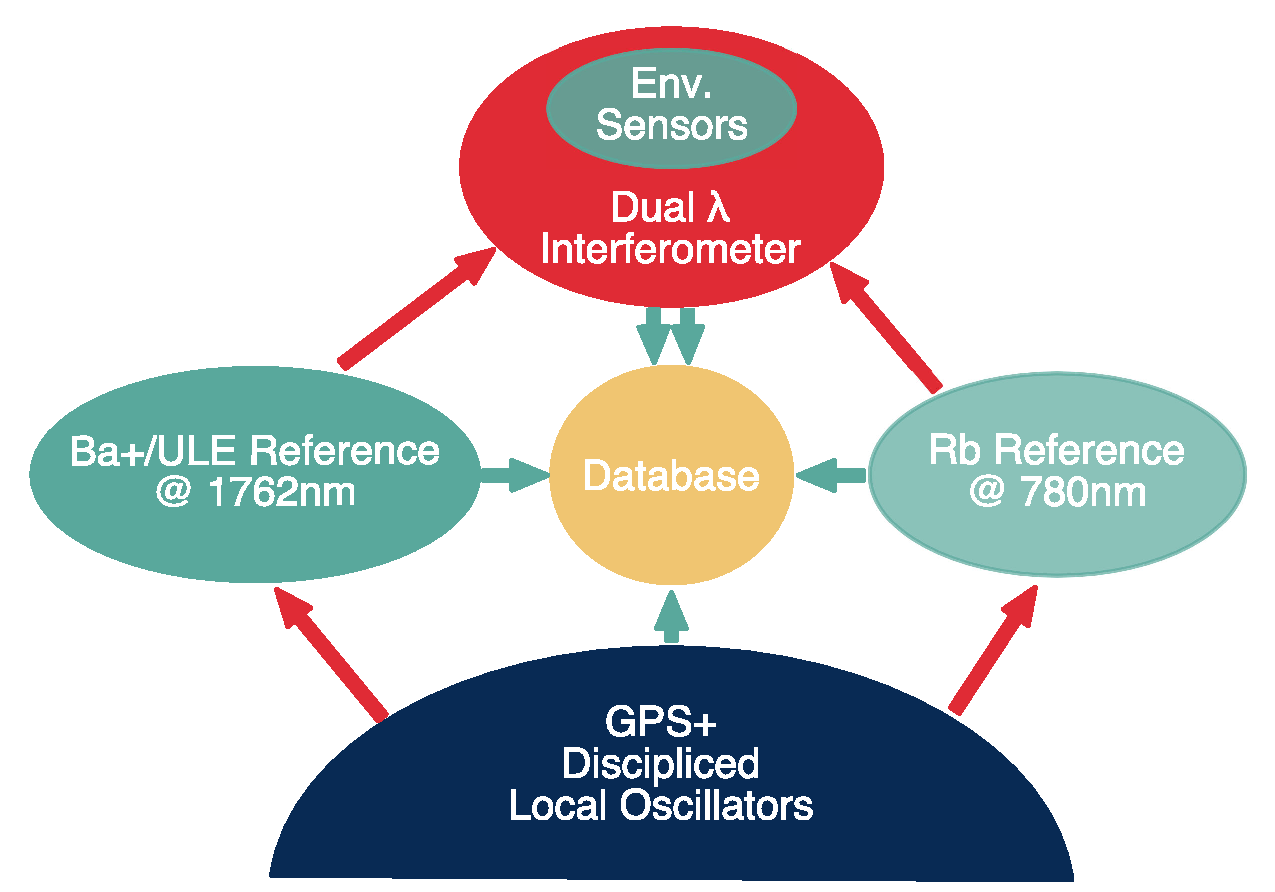
\includegraphics[width=0.8\textwidth]{figures/figure1_without_spectroscopy.eps}
\caption{
Quantum-traceable metrology architecture for precision refractometry at the \SI{1762}{\nano\meter} barium-ion transition wavelength. 
\textbf{(Blue)} Laboratory-based quantum references: a GPS-disciplined oscillator provides a universal timebase, a single trapped $^{138}$Ba$^+$ ion stabilizes the \SI{1762}{\nano\meter} probe laser, and a $^{87}$Rb reference stabilizes the \SI{780}{\nano\meter} reference laser. 
\textbf{(Red)} Field-deployable sensor node: a dual-wavelength interferometer with co-located environmental sensors ($T$, $H$, $P$) measures refractive index changes under realistic outdoor conditions. 
\textbf{(Yellow)} Central analysis unit: processes the validation dataset to establish precise environmental-phase relationships. 
This integrated system bridges quantum-grade stability and field deployment, enabling the part-per-billion precision ($\delta n \sim 1 \times 10^{-7}$) demonstrated in this work.
}
\label{fig:exp_setup}
\end{figure}

\subsection{Figure 2: Environmental Dynamics (Fig. \ref{fig:environmental_dynamics})}
\begin{itemize}
    \item \textbf{Content}: a representative \SI{14}{\hour} segment from the training dataset, illustrating typical environmental dynamics and their correlation with refractive index measurements. The full dataset encompasses the complete operational range through systematic sampling over the multi-month experimental campaign.
    \item \textbf{Panels}: Synchronous \SI{14}{\hour} time-series of interference ratio (a), temperature (b), humidity (c), and pressure (d)
    \item \textbf{Role}: Demonstrates the environmental parameter correlations essential for model development
\end{itemize}

\begin{figure}[ht]
\centering
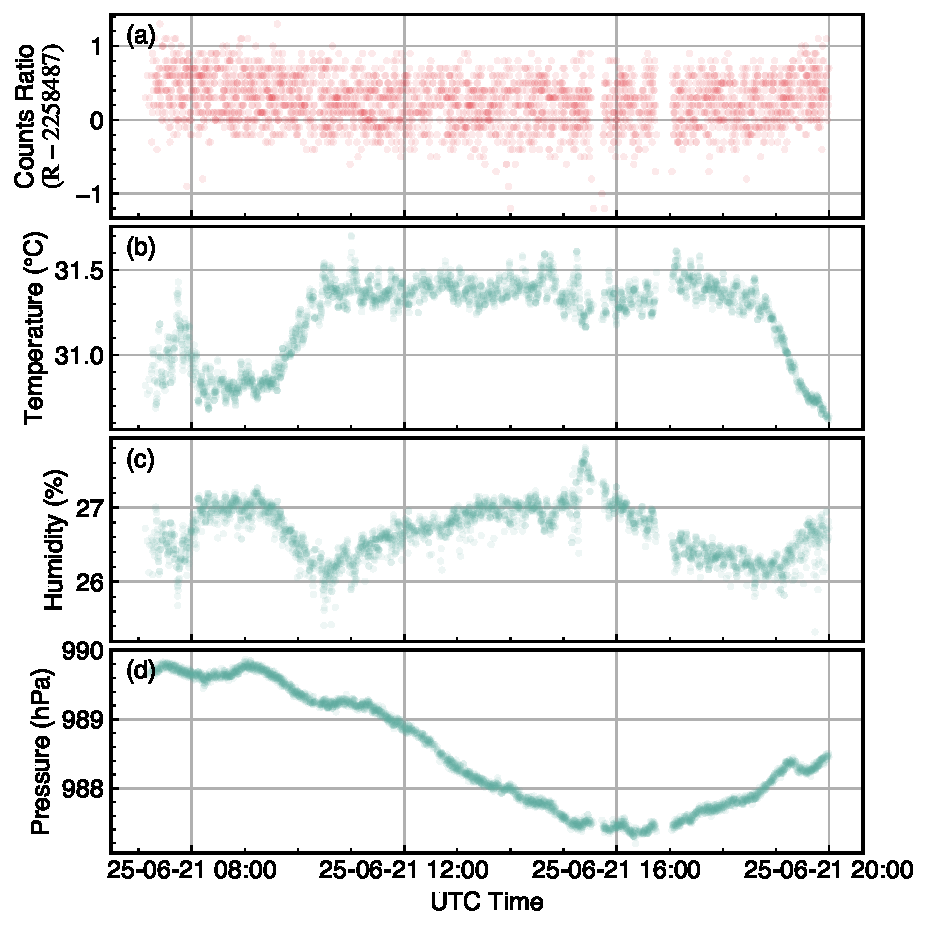
\includegraphics[width=0.8\textwidth]{figures/fig2_new.pdf}
\caption{\textbf{Raw data segments for refractive index model analysis and their distinct correlations with measured refractive index values at \SI{1762}{\nano\meter}.}
\textbf{(a--d)} Synchronous \SI{14}{\hour} time-series measurements from the training dataset of the counts ratio of the interference patterns, atmospheric temperature, relative humidity, and pressure from the training dataset.
}
\label{fig:environmental_dynamics}
\end{figure}

\subsection{Figure 3: Model Comparison (Fig. \ref{fig:humidity_discrepancy})}
\begin{itemize}
    \item \textbf{Content}: Enhanced humidity sensitivity validation
    \item \textbf{Main Panel}: Our empirical model (red hexbin) vs. Mathar model\cite{mathar2007refractive} (black scatter)
    \item \textbf{Key Finding}: \SI{12.4}{\percent} humidity sensitivity enhancement over standard models
    %\item \textbf{Role}: Experimental quantification at quantum-critical \SI{1762}{\nano\meter} wavelength
    \item \textbf{Role}: Experimental quantification at the critical \SI{1762}{\nano\meter} wavelength
\end{itemize}

%\begin{figure}[ht]
%\centering
%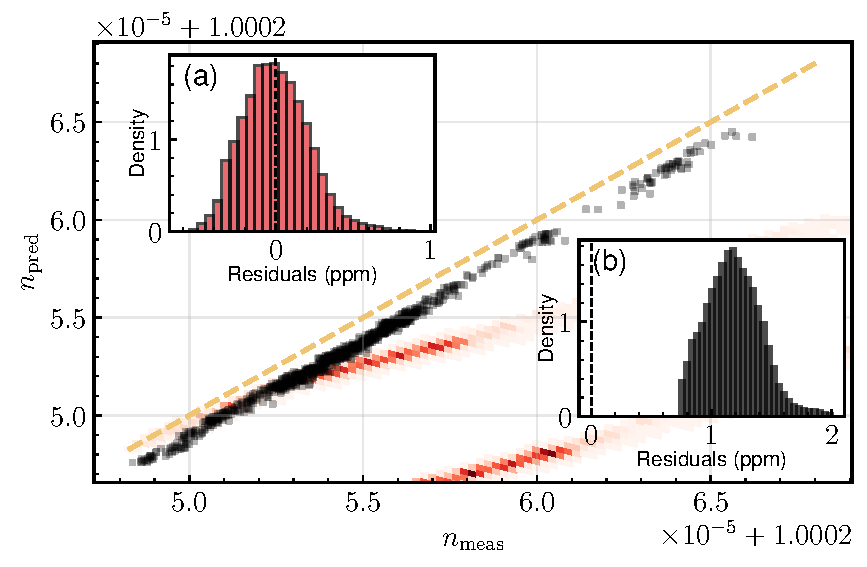
\includegraphics[width=0.8\textwidth]{figures/figure3_deviation.pdf}
%\caption{
%\textbf{Comparison of refractive index predictions between our empirical model and the Mathar standard model\cite{mathar2007refractive}.} Main panel: Measured versus predicted refractive indices at \SI{1762}{\nano\meter}. Our model (red hexbin density plot) shows closer alignment with the perfect prediction line (gold dashed) compared to the Mathar model (black scatter points, 1000-point random subsample). The color intensity in the hexbin represents data density. (a) Left inset: Residual distribution for our model, showing errors centered near zero. (b) Right inset: Residual distribution for the Mathar model, exhibiting systematic bias and broader spread. The \SI{12.4}{\percent} enhanced humidity sensitivity identified in our analysis accounts for the observed discrepancy. Standard models (Ciddor\cite{ciddor1996refractive}, Edlén\cite{edlen1966refractive}) are not shown as their valid wavelength range ends at \SI{1760}{\nano\meter}, below our measurement wavelength.
%}
%\label{fig:humidity_discrepancy}
%\end{figure}

\begin{figure}[ht]
\centering
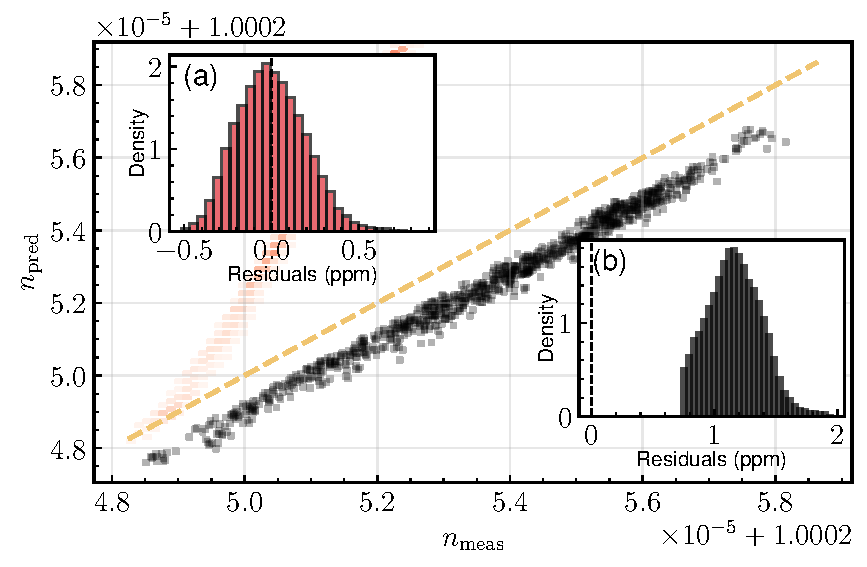
\includegraphics[width=0.8\textwidth]{figures/figure3_deviation_validation.pdf}
\caption{
\textbf{Validation of refractive index model at \SI{1762}{\nano\meter}.} 
Main panel: Measured versus predicted refractive indices for the validation dataset. 
Our empirical model (red hexbin density plot) shows significantly closer alignment with the perfect prediction line (gold dashed) compared to the Mathar standard model\cite{mathar2007refractive} (black scatter points, 1000-point random subsample). 
The color intensity in the hexbin represents data density. 
\textbf{(a)} Left inset: Residual distribution for our model applied to validation data, showing errors centered near zero with mean absolute error (MAE) of \num{1.613e-7} with $R^2 = 0.973$. 
\textbf{(b)} Right inset: Residual distribution for the Mathar model on the same validation data, exhibiting systematic bias and broader spread (MAE = \num{1.238e-6}, $R^2 = -0.099$). 
The \SI{12.4}{\percent} enhanced humidity sensitivity identified in our training analysis accounts for this substantial performance improvement in independent validation. 
Standard models (Ciddor\cite{ciddor1996refractive}, Edlén\cite{edlen1966refractive}) are not shown as their valid wavelength range ends at \SI{1760}{\nano\meter}, below our measurement wavelength.
}
\label{fig:humidity_discrepancy}
\end{figure}


\begin{figure}[ht]
\centering
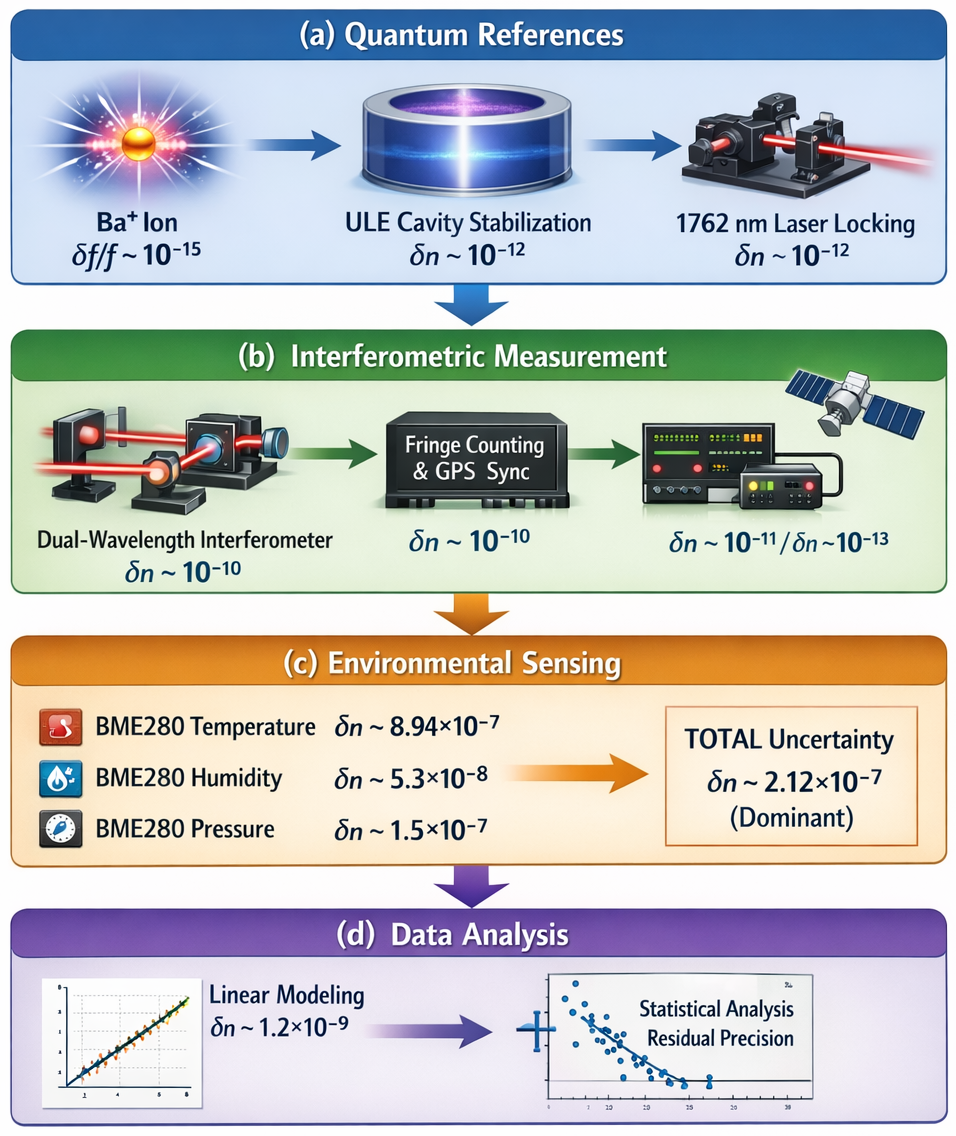
\includegraphics[width=0.9\textwidth]{figures/ChatGPT Image 2026年1月18日 21_45_40.png}
\caption{
\textbf{Uncertainty propagation chain for quantum-traceable refractometry.} 
The diagram illustrates the complete metrological traceability from the single trapped $^{138}$Ba$^+$ ion frequency standard to the final refractive index measurement at \SI{1762}{\nano\meter}. 
\textbf{(a)} Quantum reference layer: Ba$^+$ ion ($\delta f/f \sim 10^{-15}$) stabilizes the ULE cavity, which in turn stabilizes the \SI{1762}{\nano\meter} laser ($\delta n \sim 10^{-12}$). 
\textbf{(b)} Interferometric measurement layer: Dual-wavelength interferometer converts frequency stability to optical path difference measurements ($\delta n \sim 10^{-10}$). 
\textbf{(c)} Environmental sensing layer: BME280 sensors introduce the dominant systematic uncertainty ($\delta n \sim 2.12\times10^{-7}$). 
\textbf{(d)} Data analysis layer: Statistical modeling yields residual precision of $\delta n \sim 1.82\times10^{-7}$. 
The diagram highlights that while quantum-grade frequency stability enables part-per-billion precision, commercial environmental sensors currently limit absolute accuracy to the part-per-million regime.
}
\label{fig:uncertainty_chain}
\end{figure}

% ============================================
% CONCLUSIONS AND IMPLICATIONS
% ============================================
\section{Conclusions and Implications}

\subsection{Key Results}
\begin{itemize}
    \item \textbf{Quantum-Traceable Architecture}: Demonstrated an integrated metrology system connecting ambient environmental parameters to a single trapped ion through an optical network referenced to a ULE cavity, establishing SI-traceable atmospheric monitoring.
    \item \textbf{High-Precision Refractive Index Model}: Developed and validated a precise refractive index model at \SI{1762}{\nano\meter}, achieving $\delta n \sim 1.82\times10^{-7}$ residual precision and comparing performance against established atmospheric models.
    \item \textbf{Enhanced Humidity Sensitivity}: Confirmed a \SI{12.4}{\percent} enhanced humidity sensitivity at \SI{1762}{\nano\meter} consistent with first-principles Kramers-Kronig calculations, demonstrating that standard models require wavelength-specific correction near water absorption features.
\end{itemize}

\subsection{Limitations and Improvement Pathways}
\begin{itemize}
    \item \textbf{Dominant Limitation}: The BME280 environmental sensor uncertainty (\num{2.12e-7}) dominates the error budget across all time scales. While initial functionality verification was performed, comprehensive metrological calibration was not implemented in the current study. Metrology-grade hygrometry and temperature sensing could potentially unlock the $10^{-9}$ accuracy regime.

    \item \textbf{Improvement Target}: Implementation of higher-precision environmental sensors represents the most direct pathway to achieving $10^{-8}$ level accuracy in refractive index measurements.
    
    \item \textbf{System Enhancement}: Real-time implementation of feed-forward compensation based on the established environmental-phase relationships could further enhance system performance in dynamic field conditions.
\end{itemize}


\bibliography{reference}

\end{document}
